\section{Scientific Communities}


The notion of community can be understood as a dense group of nodes in a network, with more edges inside than edges linking the rest of the network.  There are multiple definitions
and strategies of identifying communities and they vary according to the context~\cite{Kleinberg@cacm2008,Leskovec@www2010}. In our context, a scientific community is defined in terms of a large and well established
scientific conference able to aggregate researchers working in similar research topics along a considerable number of years. 


In order to construct a set of scientific communities, we have gathered data from DBLP\footnote{http://dblp.uni-trier.de/}~\cite{Ley:2009}, a digital library containing more
than 2.1 million publications from 1.2 million authors that provides bibliographic information on major Computer Science conference proceedings and journals.  DBLP offers its
entire database in XML format, which facilitates gathering and constructing entire scientific communities. 

Each publication is accompanied by its title, list of authors, year of publication, and publication venue, i.e., the conference or journal. For the purposes of our work, we
consider a scientific community as a graph in which nodes represent researchers and edges links coauthors of papers from the same community.  In order to define such communities,
we focus on the publications from the flagship conferences of major ACM SIGs (Special Interest Groups).  Thus, we define a scientific community by linking people that have
coauthored a paper in a certain conference, making the flagship conferences of the ACM SIGs to act as communities where coauthorships are formed. We have removed young conferences
without enough data for a temporal analysis as well as conferences whose entire history is not registered on DBLP to allow us carrying out temporal analyses. 

In total, 24 scientific communities were constructed. Table~\ref{tab:sigs_conference_period} lists these communities, including the respective ACM SIG, the conference acronym, the period
considered (some conferences had the period reduced to avoid hiatus in the data), the total number of authors, publications and editions as well as ratios extracted from these last three figures.

\begin{table*}[!htb]
\centering
\caption{DBLP statistics on the flagship conferences of ACM SIGs}
\label{tab:sigs_conference_period}
{\small
\begin{tabular}{|l|l|c|c|c|c|c|c|c|c|} \hline
\bf{SIG} & \bf{Conference} & \bf{Period} & \bf{Authors} & \bf{Publications} & \bf{Editions} & \bf{Aut/Edi} & \bf{Pub/Edi} & \bf{Aut/Pub}\\ \hline
SIGACT & STOC & 1969-2012 & 2159 & 2685 & 44 & 49.07 & 61.02 & 0.80\\ \hline
SIGAPP & SAC & 1993-2011 & 9146 & 4500 & 19 & 481.37 & 236.84 & 2.03\\ \hline
SIGARCH & ISCA & 1976-2011 & 2461 & 1352 & 36 & 68.36 & 37.56 & 1.82\\ \hline
SIGBED & HSCC & 1998-2012 & 846 & 617 & 15 & 56.40 & 41.13 & 1.37\\ \hline
SIGCHI & CHI & 1994-2012 & 5095 & 2819 & 19 & 268.16 & 148.37 & 1.81\\ \hline
SIGCOMM & SIGCOMM & 1988-2011 & 1593 & 796 & 24 & 66.38 & 33.17 & 2.00\\ \hline
SIGCSE & SIGCSE & 1986-2012 & 3923 & 2801 & 27 & 145.30 & 103.74 & 1.40\\ \hline
SIGDA & DAC & 1964-2011 & 8876 & 5693 & 48 & 184.92 & 118.60 & 1.56\\ \hline
SIGDOC & SIGDOC & 1989-2010 & 1071 & 810 & 22 & 48.68 & 36.82 & 1.32\\ \hline
SIGGRAPH & SIGGRAPH & 1985-2003 & 1920 & 1108 & 19 & 101.05 & 58.32 & 1.73\\ \hline
SIGIR & SIGIR & 1978-2011 & 3624 & 2687 & 34 & 106.59 & 79.03 & 1.35\\ \hline
SIGKDD & KDD & 1995-2011 & 3078 & 1699 & 17 & 181.06 & 99.94 & 1.81\\ \hline
SIGMETRICS & SIGMETRICS & 1981-2011 & 2083 & 1174 & 31 & 67.19 & 37.87 & 1.77\\ \hline
SIGMICRO & MICRO & 1987-2011 & 1557 & 855 & 25 & 62.28 & 34.20 & 1.82\\ \hline
SIGMM & MM & 1993-2011 & 5400 & 2928 & 19 & 284.21 & 154.11 & 1.84\\ \hline
SIGMOBILE & MOBICOM & 1995-2011 & 1151 & 480 & 17 & 67.71 & 28.24 & 2.40\\ \hline
SIGMOD & SIGMOD & 1975-2012 & 4202 & 2669 & 38 & 110.58 & 70.24 & 1.57\\ \hline
SIGOPS & PODC & 1982-2011 & 1685 & 1403 & 30 & 56.17 & 46.77 & 1.20\\ \hline
SIGPLAN & POPL & 1975-2012 & 1527 & 1217 & 38 & 40.18 & 32.03 & 1.25\\ \hline
SIGSAC & CCS & 1996-2011 & 1354 & 676 & 16 & 84.63 & 42.25 & 2.00\\ \hline
SIGSAM & ISSAC & 1988-2011 & 1100 & 1177 & 24 & 45.83 & 49.04 & 0.93\\ \hline
SIGSOFT & ICSE & 1987-2011 & 3502 & 2248 & 25 & 140.08 & 89.92 & 1.56\\ \hline
SIGUCCS & SIGUCCS & 1989-2011 & 1771 & 1593 & 23 & 77.00 & 69.26 & 1.11\\ \hline
SIGWEB & CIKM & 1992-2011 & 4978 & 2623 & 20 & 248.90 & 131.15 & 1.90\\ \hline
\end{tabular}
}
\end{table*}





%\begin{figure*}
%\centering
%\includegraphics[scale=.4]{graficos/sigs_metricas_acumuladas_1_em_1_ano/assortatividade_grupo_temporal_web.eps}
%\caption{Assortativity accumulated from 1 in 1 year}
%\label{fig:assortativity_1_in_1}
%\end{figure*}

%\begin{figure*}
%\centering
%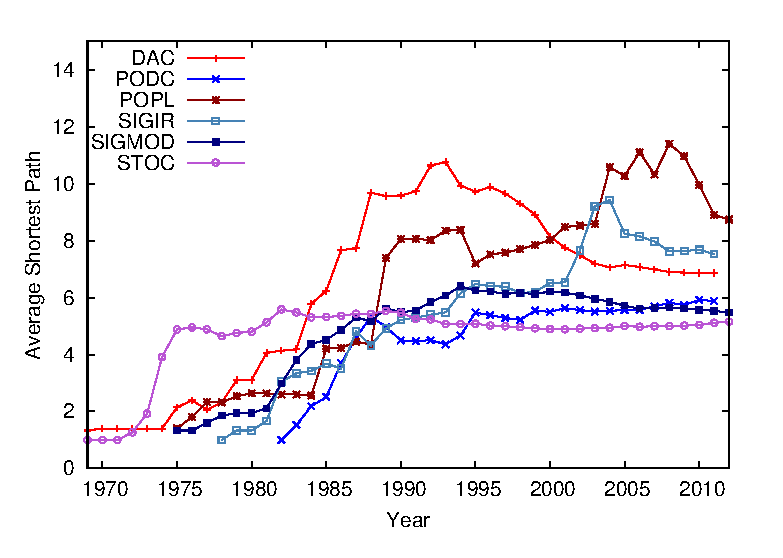
\includegraphics[scale=.4]{graficos/sigs_metricas_acumuladas_1_em_1_ano/caminho_minimo_medio_grupo_temporal_web.eps}
%\caption{Average shortest path accumulated from 1 in 1 year}
%\label{fig:average_shortest_path_1_in_1}
%\end{figure*}

%\begin{figure*}
%\centering
%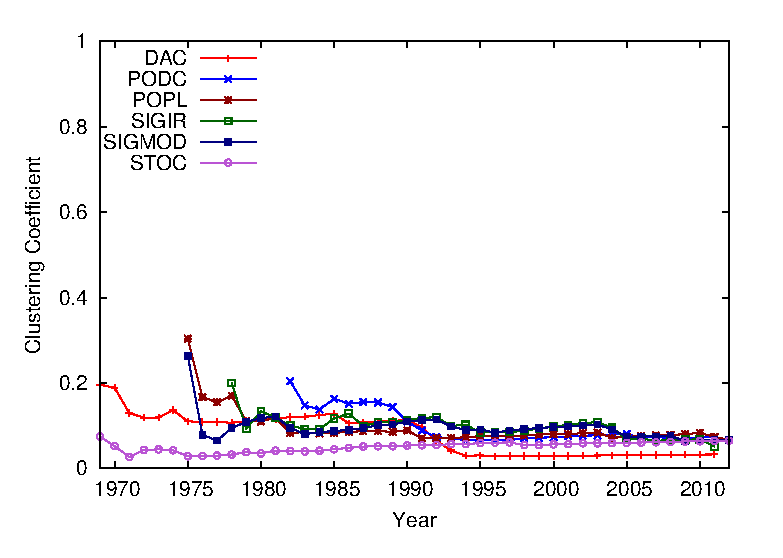
\includegraphics[scale=.4]{graficos/sigs_metricas_acumuladas_1_em_1_ano/coeficiente_agrupamento_grupo_temporal_web.eps}
%\caption{Clustering Coefficient accumulated from 1 in 1 year}
%\label{fig:clustering_coefficient_1_in_1}
%\end{figure*}

%\begin{figure*}
%\centering
%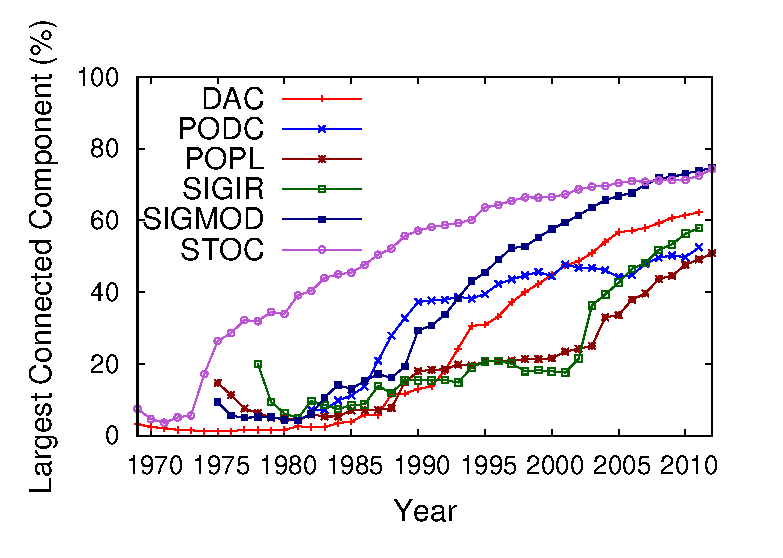
\includegraphics[scale=.4]{graficos/sigs_metricas_acumuladas_1_em_1_ano/porcentagem_maior_componente_grupo_temporal_web.eps}
%\caption{Largest connected component accumulated from 1 in 1 year}
%\label{fig:largest_connected_component_1_in_1}
%\end{figure*}



